\chapter{Nintendo's Response and Industry Implications}
\epigraph{quote}{\textit{author}}

\section{Mitigation Efforts}

\subsection{Hardware Revisions}
In response to the Fusee Gelee exploit, Nintendo undertook several significant hardware revisions to mitigate the vulnerability. The primary strategy involved modifying the Boot ROM code in newer models of the Nintendo Switch. This entailed introducing an updated version of the Tegra X1 chip, known as the "Mariko" chip.\cite{SwitchSystemFlaws} The Mariko chip features a corrected Boot ROM that addresses the buffer overflow vulnerability exploited by Fusee Gelee. Consequently, Nintendo released new hardware models incorporating this updated Tegra X1 chip, such as the Switch Lite and the revised standard Switch. These models are immune to the specific Fusee Gelee exploit, as the vulnerability in the Boot ROM has been patched.
\subsection{Software Updates}
Nintendo also implemented software updates to enhance the overall security of the system and address potential vulnerabilities. Regular firmware updates were deployed to improve the security features of the Switch operating system, including fixes for known software vulnerabilities and enhancements to the system's security architecture. These updates introduced improved cryptographic checks and integrity verification processes to strengthen the console's defenses against unauthorized access.


\section{Effectiveness and Critique}

\subsection{Evaluation of Hardware Revisions}
The hardware revisions implemented by Nintendo have proven effective in mitigating the specific vulnerability exploited by Fusee Gelee. The introduction of the Mariko chip and the release of new hardware models have successfully prevented this exploit from being executed on these devices. However, this approach has certain limitations.

Firstly, requiring consumers to purchase new hardware to benefit from these security improvements imposes a financial burden, which may not be feasible for all users. Secondly, older models of the Switch remain vulnerable to the exploit, posing a continued security risk for users who have not upgraded their hardware.

Even though the Boot ROM vulnerability has been addressed in the Mariko chip, the new consoles are still susceptible to hacking, albeit through more complex methods. Other potential hardware vulnerabilities exist in different components of the Switch. These vulnerabilities require a more sophisticated attack vector to exploit, often involving additional tools such as a Raspberry Pi and soldering equipment. This increased complexity raises the barrier to entry for potential hackers but does not entirely eliminate the risk.\cite{wololoHowHackYour2023}

\begin{figure}[H]
    \centering
    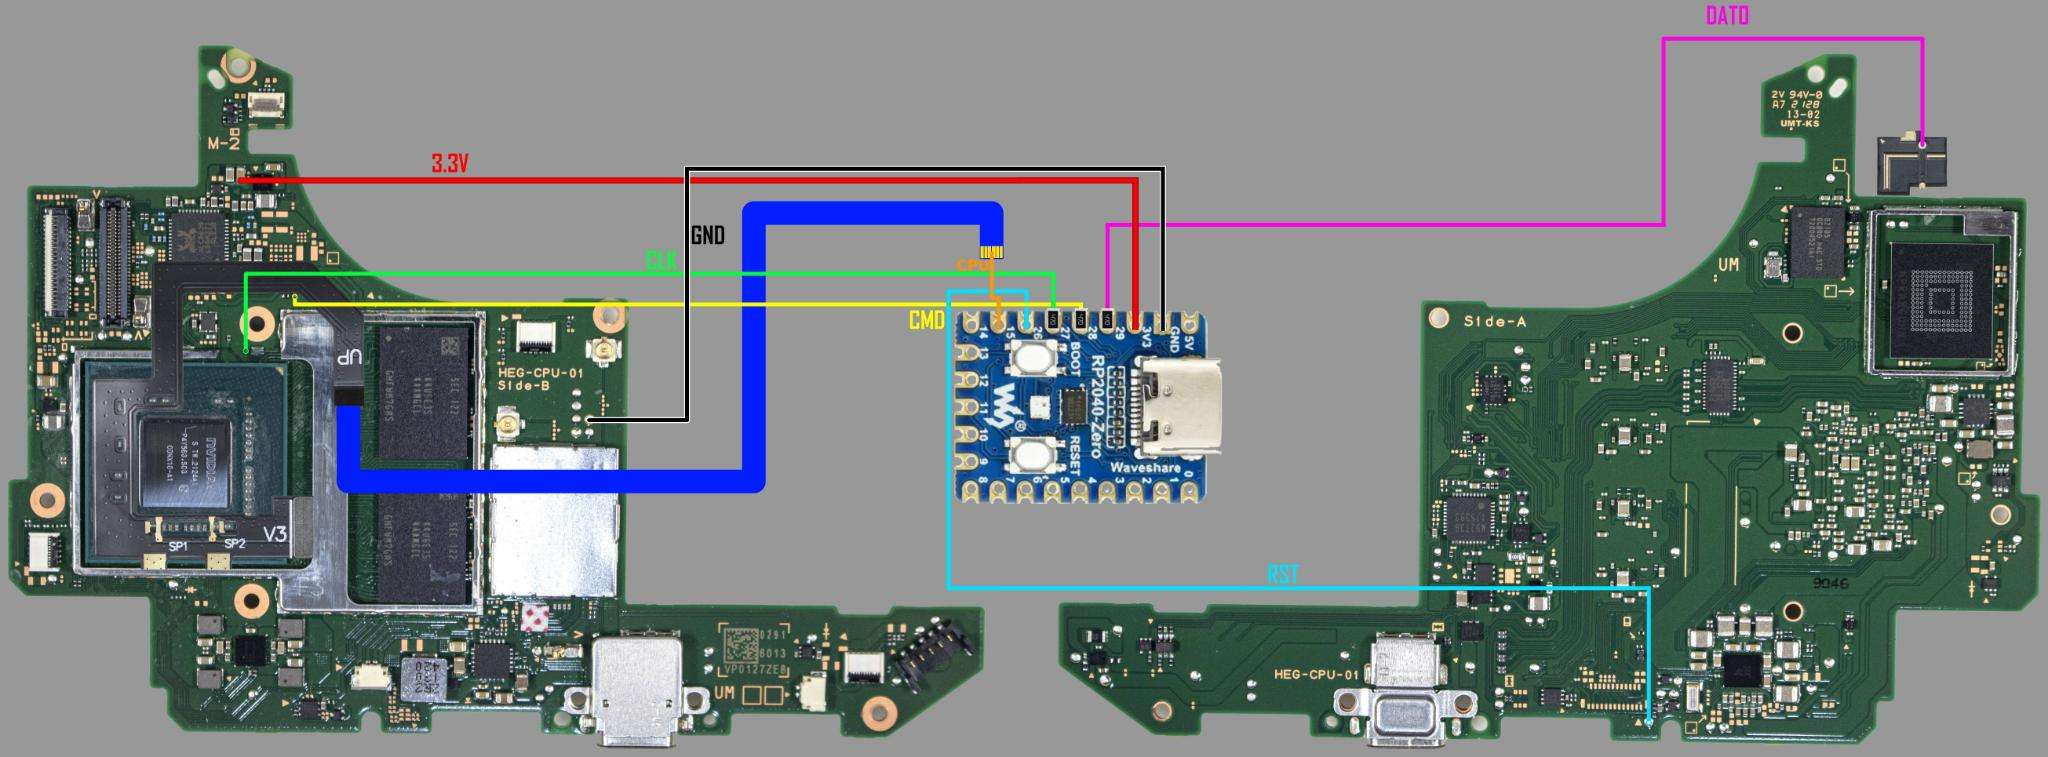
\includegraphics[width=.8\linewidth]{images/picofly_board.jpg}
    \caption{Hacking the latest Nintendo Switch models using the Picofly board\cite{PicoflyAIOThread}}
    \label{fig:switch_boot}
\end{figure}

\subsection{Critique of Software Updates}
While software updates play a crucial role in enhancing security, they have inherent limitations in addressing hardware vulnerabilities. The effectiveness of software updates relies heavily on user compliance; users who neglect to update their devices remain vulnerable to known exploits. Furthermore, software patches alone cannot fix vulnerabilities embedded in immutable hardware components like the Boot ROM.
\subsection{Overall Impact on Security Posture}
Despite these limitations, Nintendo's combined approach of hardware revisions and software updates has significantly improved the security posture of the Nintendo Switch. By addressing both immediate vulnerabilities and enhancing overall system security, Nintendo has demonstrated a proactive stance in managing hardware security risks. However, the ongoing challenge of maintaining security in the face of evolving threats underscores the need for continuous vigilance and robust security practices in the design and maintenance of hardware systems.